\documentclass[conference]{IEEEtran}
\usepackage{cite}
\usepackage{amsmath,amssymb,amsfonts}
\usepackage{algorithm}
\usepackage{algorithmic}
\usepackage{graphicx}
\usepackage{textcomp}
\usepackage{xcolor}
\usepackage{booktabs}
\usepackage{array}
\usepackage{tabularx}
\usepackage{url}
\newcolumntype{Y}{>{\raggedright\arraybackslash}X}

\newcommand{\pcqv}{PCQV}
\newcommand{\ctx}{\gamma}
\newcommand{\sem}[1]{\mathopen{[\![}#1\mathclose{]\!]}}
\newcommand{\prot}[1]{#1^{P,\ctx}}
\newtheorem{theorem}{Theorem}
\newtheorem{lemma}{Lemma}
\newtheorem{definition}{Definition}

\begin{document}

\title{Visibility Capsules for Efficient and Certified Policy-Constrained Query Optimization}

\author{%
\IEEEauthorblockN{Haoyi Zhang and Huaijin Ran}
\IEEEauthorblockA{\textit{Xi'an Jiaotong-Liverpool University}\\
Suzhou, China\\
hyeliozhang@gmail.com, seventeen17510@gmail.com}
}

\maketitle
% Auto-generated by artifact/pcqv/engine.py summarize().
\newcommand{\NumPerformanceRows}{4320}
\newcommand{\NumCorrectnessRows}{1152}
\newcommand{\NumAblationRows}{1008}
\newcommand{\NumCardinalityRows}{1230}
\newcommand{\SafeEqPassed}{1064}
\newcommand{\SafeEqTotal}{1064}
\newcommand{\UnsafeViolations}{3816}
\newcommand{\PcqvMedianMs}{0.413}
\newcommand{\PcqvSpeedView}{2.74}
\newcommand{\PcqvSpeedPost}{1.308}
\newcommand{\PcqvSpeedObliv}{1.416}
\newcommand{\PcqvPredRatio}{1.025}
\newcommand{\PcqvCompileMs}{0.157}
\newcommand{\PolicyQErrorMedian}{1.139}
\newcommand{\PolicyQErrorPninetyfive}{3.5}

\newcommand{\PerfSummaryRows}{%
post\_join\_filter & 0.714 & 6.268\\
view\_barrier & 1.439 & 15.234\\
oblivious\_forced & 0.688 & 7.285\\
predicate\_injection & 0.428 & 6.152\\
pcqv\_no\_stats & 0.378 & 6.11\\
pcqv\_forced & 0.414 & 6.317\\
pcqv & 0.413 & 6.369\\
oracle\_order & 0.42 & 5.692\\
}
\newcommand{\ByQueryRows}{%
q10\_acl\_customer\_rows & 0.171 & 0.254 & 0.158 & 0.193 & 0.124 & 0.087\\
q11\_order\_ticket\_bridge & 0.434 & 0.775 & 0.493 & 0.434 & 0.472 & 0.51\\
q12\_product\_segment\_revenue & 0.881 & 3.324 & 0.755 & 0.652 & 0.496 & 0.775\\
q13\_order\_lineitem\_rows & 0.854 & 2.572 & 0.929 & 0.891 & 1.116 & 1.111\\
q14\_support\_owner\_rows & 0.341 & 0.441 & 0.29 & 0.246 & 0.217 & 0.236\\
q15\_clearance\_product\_rows & 0.473 & 2.364 & 0.339 & 0.322 & 0.411 & 0.416\\
q16\_region\_product\_mix & 0.856 & 3.451 & 0.824 & 0.742 & 0.994 & 0.621\\
q1\_customer\_orders & 0.733 & 2.554 & 0.941 & 0.29 & 0.426 & 0.336\\
q2\_revenue\_by\_product & 1.011 & 3.412 & 1.658 & 0.665 & 0.473 & 0.411\\
q3\_support\_tickets & 0.213 & 0.474 & 0.247 & 0.157 & 0.13 & 0.208\\
q4\_revenue\_by\_region & 0.881 & 3.927 & 1.729 & 0.783 & 0.851 & 0.649\\
q5\_high\_value\_segments & 1.956 & 0.502 & 1.988 & 2.03 & 1.668 & 1.423\\
q6\_lineitem\_product\_count & 1.53 & 3.696 & 2.084 & 0.707 & 0.622 & 0.737\\
q7\_customer\_summary & 0.386 & 0.612 & 0.4 & 0.173 & 0.181 & 0.254\\
q8\_sensitive\_product\_scan & 1.736 & 2.878 & 1.73 & 0.864 & 0.89 & 0.883\\
q9\_ticket\_topic\_segments & 0.401 & 0.583 & 0.344 & 0.288 & 0.327 & 0.347\\
}
\newcommand{\BySelectivityRows}{%
0.025 & 0.167 & 0.062 & 0.178 & 0.053 & 0.055 & 0.069\\
0.05 & 0.241 & 0.674 & 0.289 & 0.118 & 0.115 & 0.142\\
0.1 & 0.574 & 2.272 & 0.498 & 0.374 & 0.384 & 0.365\\
0.25 & 1.677 & 6.024 & 1.751 & 1.195 & 1.102 & 1.265\\
0.5 & 2.823 & 11.901 & 3.472 & 2.589 & 2.556 & 2.607\\
}
\newcommand{\ByComplexityRows}{%
1 & 1.057 & 2.377 & 1.254 & 0.942 & 1.024 & 0.792\\
2 & 0.867 & 1.852 & 0.878 & 0.45 & 0.473 & 0.424\\
3 & 0.491 & 1.062 & 0.483 & 0.291 & 0.223 & 0.257\\
4 & 0.563 & 1.473 & 0.604 & 0.229 & 0.261 & 0.339\\
5 & 0.585 & 1.255 & 0.602 & 0.32 & 0.326 & 0.368\\
6 & 0.5 & 1.28 & 0.617 & 0.384 & 0.329 & 0.361\\
}
\newcommand{\AblationRows}{%
oblivious\_forced & 1.175\\
oracle\_order & 0.765\\
pcqv & 0.792\\
pcqv\_forced & 0.761\\
pcqv\_greedy & 0.709\\
pcqv\_no\_order & 0.768\\
pcqv\_no\_stats & 0.717\\
}

% Auto-appended by certificate_counterexample_audit.py.
\newcommand{\CertRules}{8}
\newcommand{\CertCases}{528}
\newcommand{\CertAccepted}{264}
\newcommand{\CertRejected}{264}
\newcommand{\CertUnsafeWitnesses}{36}

% Auto-appended by capsule_minimality_audit.py and statistical_confidence_audit.py.
\newcommand{\CapsuleFieldsTested}{8}
\newcommand{\CapsuleNecessaryFields}{8}
\newcommand{\CapsuleWitnessDiffs}{13}
\newcommand{\CapsuleWitnessViolations}{3}
\newcommand{\MainSpeedViewCILow}{2.37}
\newcommand{\MainSpeedViewCIHigh}{3.03}
\newcommand{\JobSpeedViewCILow}{2.48}
\newcommand{\JobSpeedViewCIHigh}{7.65}
\newcommand{\PcqvCompileCILow}{0.135}
\newcommand{\PcqvCompileCIHigh}{0.219}

% Auto-appended by grandfinal audits.
\newcommand{\MultiSeedFuzzSeeds}{4}
\newcommand{\MultiSeedFuzzRows}{2400}
\newcommand{\MultiSeedFuzzSafeEq}{960}
\newcommand{\MultiSeedFuzzSafeTotal}{960}
\newcommand{\MultiSeedFuzzDiffs}{37168}
\newcommand{\MultiSeedFuzzViolations}{24877}
\newcommand{\PortableSQLGenerated}{6048}
\newcommand{\PortableSQLPlanNodes}{37591}
\newcommand{\PortableSQLIndexPlans}{6042}
\newcommand{\CodeAuditPyFiles}{31}
\newcommand{\CodeAuditTotalLines}{6597}

% Auto-appended by proof_carrying_rewrite_suite.py.
\newcommand{\ProofCertSafeAccepted}{1064}
\newcommand{\ProofCertSafeTotal}{1064}
\newcommand{\ProofCertRejected}{424}
\newcommand{\ProofCertRows}{1488}
\newcommand{\ProofCertObligations}{28}
\newcommand{\ProofCertMandatoryCovered}{18}
% Generated by paired comparison audit.
\newcommand{\MainPairedCells}{480}
\newcommand{\PcqvViewWins}{437}
\newcommand{\PcqvViewWinPct}{91.0}
\newcommand{\PcqvPostWins}{353}
\newcommand{\PcqvPostWinPct}{73.5}
\newcommand{\PcqvOblivWins}{359}
\newcommand{\PcqvOblivWinPct}{74.8}
\newcommand{\PcqvPredWins}{265}
\newcommand{\PcqvPredWinPct}{55.2}


% Generated by manuscript consistency audit.
\newcommand{\JobPairedSpeedView}{2.753}

\newcommand{\RandomFuzzTemplates}{240}

\newcommand{\RandomFuzzRows}{3600}

\newcommand{\RandomFuzzSafeEq}{1440}

\newcommand{\RandomFuzzSafeTotal}{1440}

\newcommand{\RandomFuzzDiffs}{60445}

\newcommand{\RandomFuzzViolations}{39485}

\newcommand{\OptimizerSearchCases}{150}

% Auto-appended by optimizer_search_audit.py.
\newcommand{\OptimizerSearchSuboptimal}{74}
\newcommand{\OptimizerSearchMaxRegret}{4.958}
\newcommand{\OptimizerSearchMaxAliases}{8}
\newcommand{\OptimizerSearchMaxOrders}{40320}
% Auto-appended by efficiency_scalability_audit.py.
\newcommand{\ScaleSweepRows}{600}
\newcommand{\ScaleSweepSizes}{5}
\newcommand{\ScaleLargestPcqvMs}{2.308}
\newcommand{\ScaleLargestInjectionMs}{3.829}
\newcommand{\ScaleLargestObliviousMs}{5.963}
\newcommand{\ScaleLargestViewMs}{26.678}
\newcommand{\ScaleLargestViewSpeedup}{11.560}
\newcommand{\ScaleLargestInjectionRatio}{1.659}
\newcommand{\ScaleSummaryRows}{%
0.03 & 0.593 & 0.600 & 0.920 & 3.780\\
0.06 & 0.559 & 0.588 & 0.916 & 3.677\\
0.12 & 0.769 & 0.840 & 1.372 & 6.112\\
0.24 & 1.437 & 1.710 & 2.939 & 12.675\\
0.48 & 2.308 & 3.829 & 5.963 & 26.678\\
}
% Auto-appended by memo_integration_audit.py.
\newcommand{\MemoCandidateRecords}{6048}
\newcommand{\MemoAliasPropertyRecords}{15498}
\newcommand{\MemoCrossDependencyRecords}{2772}
\newcommand{\MemoReleaseGuardRecords}{693}
\newcommand{\MemoMaskObligationRecords}{3024}
\newcommand{\MemoProfileCount}{3}



\begin{abstract}
Policy-aware analytics often force a difficult choice: protected views keep the semantics explicit but can hide useful optimization state, while injected predicates are fast only when the optimizer is allowed to treat policy predicates as ordinary filters. This paper proposes Policy-Constrained Query Visibility (\pcqv), a query-optimization interface based on \emph{visibility capsules}. A capsule records the optimizer-facing policy facts that affect relational rewrites: alias-local guards, cross-alias dependencies, masks, release guards, deterministic-order obligations, and protected selectivity. The compiler uses these fields to certify safe rewrites and to expose protected cardinality to a Selinger-style planner; each emitted plan carries a local certificate that is checked against a protected-view reference semantics.

A portable Python/SQLite artifact implements the compiler, planner, baselines, unsafe mutation controls, finite-model checks, SQL-feature checks, randomized fuzzing, memo-property bridge records, and claim-level reproducibility gates. The evaluation emphasizes efficiency and scalability rather than only correctness: the main benchmark contains 4,320 timing measurements and 1,064/1,064 safe equivalence checks; a five-size scale sweep adds \ScaleSweepRows{} measurements; TPC-H/SSB-style and JOB/IMDb-style stress tests add 204/204 safe equivalence checks. Across paired main-workload cells, \pcqv{} is \PcqvSpeedView{}$\times$ faster than protected-view barriers; at the largest scale point it is \ScaleLargestViewSpeedup{}$\times$ faster; and on the JOB/IMDb-style paired benchmark it is \JobPairedSpeedView{}$\times$ faster. Negative controls expose 12,863 fixed-template and \RandomFuzzDiffs{} randomized symmetric differences, while independent audits generate \PortableSQLGenerated{} safe SQL plans and \MemoCandidateRecords{} optimizer-property records. The result is a compact, certifying optimizer contract for policy-constrained query processing.
\end{abstract}

\begin{IEEEkeywords}
Query optimization, query rewriting, data security and privacy, row-level security, policy-constrained semantics, cardinality estimation, testing, benchmarking.
\end{IEEEkeywords}

\section{Introduction}
Access-control and privacy policies are no longer rare administrative filters. A single analytical query may be evaluated under row-level tenant isolation, column-level masking, purpose limitation, consent exceptions, view-based security, secure predicate pushdown restrictions, and aggregation thresholds. Modern data platforms therefore face a problem that is fundamentally about data engineering rather than only about security: the optimizer must transform and cost queries in a space where the semantics of a tuple depends on policy and context. When that semantics is hidden behind views, user-defined guards, or external enforcement code, an optimizer may lose important cardinality information. When policy predicates are pushed, delayed, or removed as if they were ordinary filters, a rewrite that is valid for plain relational algebra may cease to preserve protected results.

Classical query optimizers are built around equivalence rules, cardinality estimates, and plan enumeration\cite{selinger1979access,graefe1993volcano,graefe1995cascades,chaudhuri1998overview}. Decades of work have made such optimizers extensible, cost-based, and increasingly robust to estimation error\cite{stillger2001leo,babcock2005robust,leis2015job,marcus2021bao,yang2022balsa}. A parallel line of database work studies fine-grained authorization, predicated grants, privacy policies, and secure query modification\cite{stonebraker1974access,griffiths1976authorization,rizvi2004fgac,kabra2006redundancy,agrawal2005privacy,chaudhuri2007predicated}. Recent production systems confirm that safe and performant data access control is a query-processing concern at scale\cite{paduroiu2024membrane,xue2023sparkac,xue2020guardspark,dar2023rls}. However, the interface between these lines remains brittle. Security mechanisms often express policies as protected views or injected predicates, while optimizers treat them as ordinary SQL or as opaque barriers. Existing SQL-equivalence and database-testing tools target ordinary SQL rewrites or engine bugs\cite{chu2017cosette,chu2017hottsql,zhou2019symbolic,ding2024lia,wang2024qed,rigger2020norec,ba2024dqp}. They do not directly model the policy objects studied here: row masks, purpose contexts, and aggregate guards.

This paper studies the following question: \emph{What compact optimizer-visible contract makes policy-constrained rewrites fast, checkable, and falsifiable?} We use software-security examples as motivation, but the contribution is deliberately data-engineering-first. The system treats policies as semantic and statistical constraints on relational query processing and exposes them to the same optimizer machinery that handles algebraic equivalence, cardinality, and plan choice. The target is the missing optimizer interface behind the debugging gap: policy-constrained queries can be correct but slow, fast but unsafe, or difficult to diagnose because the policy semantics is absent from plan enumeration and testing.

The paper makes five contributions aimed at query optimization rather than policy administration. First, it defines protected relational semantics for row guards, masks, cross-table guard predicates, and aggregate-release guards, giving a reference point for policy-preserving rewrites. Second, it introduces visibility capsules and rule-level certificates for predicate movement, view elision, join reordering, mask placement, semijoins, deterministic prefixes, and aggregate boundaries; erasing any of the \CapsuleFieldsTested{} audited fields yields an executable counterexample. Third, it gives a policy-aware Selinger-style planner that exposes protected selectivity as optimizer state while separating semantic admissibility from plan choice. Fourth, it builds a portable Python/SQLite artifact with a policy compiler, safe and unsafe encodings, proof-obligation tests, a protected-view oracle, finite-model audits, SQL-feature audits, randomized fuzzing, optimizer-property bridge records, and rerunnable claim checks. Fifth, it evaluates efficiency and scalability through latency, correctness, negative controls, a five-size scale sweep, policy complexity, planning overhead, ablations, and TPC-H/SSB-style and JOB/IMDb-style stress tests. The empirical claim is that, on the reported workloads, exposing policy semantics lets certified safe optimizers recover a substantial fraction of the overhead introduced by barriers and policy-oblivious plans while keeping the rewrite boundary locally checkable and reproducible.

\section{Policy-Constrained Query Optimization}
\label{sec:problem}

\noindent\textbf{Data-engineering scope.}
The work sits at the intersection of data models, query languages, query processing, query optimization, benchmarking, testing, and data security/privacy. The core object is a relational query plan, not an authorization protocol. The questions are: what is the semantics of a protected relational expression, which rewrite rules preserve it, how should cardinality and cost reflect policy predicates, and how can an optimizer implementation be tested for policy-constrained equivalence? This aligns with established database research on query rewrite\cite{levy1994predicate,chaudhuri1995views,goldstein2001views}, view-based answering\cite{levy1995views,halevy2001views,pottinger2001minicon}, cardinality estimation\cite{leis2015job,dutt2019selectivity,kipf2019learnedcards}, and fine-grained database authorization\cite{rizvi2004fgac,kabra2006redundancy,chaudhuri2007predicated}.

\noindent\textbf{Running example.}
Consider a revenue query that joins \textit{lineitem}, \textit{orders}, and \textit{customers}, groups by customer region, and reports order counts and revenue. Without policies, an optimizer can freely choose a join order, push the date predicate into \textit{orders}, and aggregate after the joins. Under a policy context, the same query has a different optimization space. Customer rows are restricted to allowed tenants and regions; order rows must be non-internal and match the current purpose; line items must refer to permitted orders; and aggregate groups may be released only after the contributing rows have been filtered. A protected-view barrier is easy to reason about, but it may hide useful selectivity from the optimizer. A predicate-injection plan can be fast, but it must not move aggregation before row guards. A post-filter plan is semantically correct only when it carries enough raw attributes to evaluate every policy after the join, but it may create large intermediate tuples.

This example illustrates the optimizer-policy mismatch. The security requirement is not merely ``block unauthorized rows.'' The data-engineering requirement is to preserve a protected relational semantics while selecting an efficient query plan. The query optimizer must know whether a guard is local or cross-table, whether a mask is an output transformation or a predicate operand, whether an aggregate group guard constrains contributors or only outputs, and whether a policy predicate changes cardinality enough to justify a different join order.

\noindent\textbf{SQL-core fragment.}
\pcqv{} targets a SQL-core fragment that is broad enough to contain the optimizer phenomena studied in the paper while remaining auditable. Queries contain selections, inner equi-joins, semijoins, projections, deterministic scalar expressions, masks over selected columns, grouping, distributive and algebraic aggregates, having clauses, order by, limits, and view expansion. Policies are deterministic SQL predicates parameterized by an execution context. Context includes user id, role, purpose, clearance, allowed tenants, allowed regions, ACL exceptions, and a minimum group size. The main benchmark uses five base tables; the external-validity study adds a TPC-H/SSB-style decision-support schema with customer, order, lineitem, part, supplier, nation, and region tables.

The core soundness theorem is deliberately stated for the analytical SPJAG fragment--selection, projection, deterministic scalar expressions, inner joins, semijoins, grouping, aggregates, protected views, masks, row guards, and group-release guards. The prototype then extends the \emph{audit surface}, not the theorem by assertion, to SQL features that frequently break naive policy rewrites: NULL/three-valued predicates, left-outer null extension, bag duplicates, UNION ALL branch placement, antijoins, EXCEPT-style differences, HAVING, and ORDER/LIMIT with deterministic keys. Operators such as recursion, updates, nondeterministic UDFs, timing channels, and concurrent policy changes are not silently folded into the same theorem; they enter only by the same discipline: define the protected denotation, state the rewrite side condition, expose the required capsule field, and add a witness-generating obligation.


\noindent\textbf{Optimizer contract.}
A useful way to distinguish this work from an access-control implementation is to state the optimizer contract explicitly. A policy-aware optimizer receives ordinary relational structure plus policy metadata and must return SQL whose result is the protected query result, not merely a query that happens to filter unauthorized rows on one database. In \pcqv{}, every admitted transformation is also certifying: it carries a compact record of the alias bundle, guard class, value-state transition, group-release position, and deterministic-order obligation that made the transformation legal. The contract has three parts. First, policy clauses are attached to relation aliases and cannot be lost during enumeration. Second, value-changing clauses such as masks are part of the output semantics and must not be treated as ordinary selections. Third, aggregate release constraints are applied after contributor filtering, so an optimizer cannot commute them with row guards without a proof obligation.

This contract is deliberately phrased in terms familiar to query optimizers: aliases, cardinalities, rewrite side conditions, and result equivalence. It does not require a new administrative language for granting privileges. A DBMS that already stores row filters, masking expressions, and purpose labels could expose the same contract to its optimizer. Conversely, a system that enforces policies outside the optimizer can still use the checker to detect whether its generated SQL respects the protected semantics.

\begin{table}[t]
\centering
\caption{Visibility-capsule fields required by the optimizer contract.}
\label{tab:contract}
\begin{tabular}{p{0.25\columnwidth}p{0.47\columnwidth}}
\toprule
Capsule field & Optimizer obligation \\
\midrule
Tenant guard & attach base visibility to every alias \\
Purpose guard & preserve context-sensitive row predicates \\
Region guard & expose geography selectivity and scope \\
ACL exception & keep disjunctive authorization branches \\
Cross-alias guard & preserve semijoin/join dependency scope \\
Mask timing & delay masks until raw consumers finish \\
Group release & protect contributor multisets before release \\
Deterministic order & preserve protected ORDER/LIMIT prefixes \\
\bottomrule
\end{tabular}
\end{table}

\noindent\textbf{Baselines and failure modes.}
Table~\ref{tab:baselines} summarizes the baselines. They are chosen to separate enforcement choices from optimizer choices. \textit{No policy} is not a safe baseline; it measures the cost of the unprotected query only. \textit{Post-filter} materializes or logically creates a raw joined record and filters it late. \textit{Predicate injection} inserts policy predicates into the query and lets SQLite optimize. \textit{View barrier} enforces each table through a protected common table expression. \textit{Oblivious forced order} applies policies but preserves the input join order. \pcqv{} chooses among safe physical encodings using policy selectivity. \textit{Unsafe late aggregate} is a negative control that aggregates before row policies.

\begin{table}[t]
\centering
\caption{Execution methods evaluated. Only the no-policy and unsafe-late-aggregate rows are semantically unsafe diagnostic references.}
\label{tab:baselines}
\begin{tabular}{lll}
\toprule
Method & Role & Key behavior \\
\midrule
No policy & diagnostic & plain SQL, no protection \\
Post-filter & baseline & join first, filter raw tuples late \\
Injection & baseline & add guards to WHERE \\
View barrier & baseline & protected CTE per table \\
Oblivious & baseline & policies, input join order \\
\pcqv{} & proposed & policy-aware safe choice \\
Unsafe aggregate & unsafe diag. & aggregate before row guards \\
\bottomrule
\end{tabular}
\end{table}


\section{Policy-Constrained Semantics}
\label{sec:semantics}

We now define the protected semantics that the optimizer must preserve. The database question is concrete: given protected relational semantics, which transformations remain legal, which safe encodings should be costed, and which emitted queries can be checked against a protected-view reference?

Let $I$ be a relational instance, $\ctx$ an execution context, and $P$ a policy program. For each base relation $R$, $P$ defines a row guard $\rho_R(t,\ctx,I)$, optional mask functions $\mu_{R,a}(t,\ctx)$ for attributes $a$, optional cross-table guards expressible as semijoin predicates, and an optional aggregate group guard $g_Q(G,\ctx)$ for query $Q$. In the prototype all guards compile to SQLite predicates, but the semantics is independent of SQLite.

\subsection{Policy Language}
A policy program is a finite set of guarded clauses. A row clause has the form $(R,a,\phi,s)$, where $R$ is a relation, $a$ is the alias to which the clause is attached, $\phi$ is a SQL-expressible predicate over $a$, context constants, and allowed semijoin subqueries, and $s$ is a selectivity hint. A mask clause has the form $(R.a,\eta)$, where $\eta$ is a deterministic expression that can depend on the row and context. A group clause has the form $(Q,\psi)$, where $\psi$ is a having predicate such as \textit{COUNT(*) >= min\_group}. This language is small enough to compile without a parser generator, but it separates the concepts an optimizer must reason about: row elimination, value transformation, cross-table membership, and aggregate release.

Policy clauses are context dependent but not user-input strings. The prototype constructs contexts from a typed record: user id, role, purpose, clearance, allowed tenants, allowed regions, and minimum group size. This design avoids SQL-injection concerns and keeps the paper focused on optimization. In a production engine, the same policy clauses could be compiled from a governance catalog, but the optimizer-facing interface would be similar: each protected alias contributes predicates, masks, selectivity hints, and safety restrictions.


\textbf{Protected relations.} A protected base relation is
\begin{equation}
\prot{R} = \{\, t \in R \mid \rho_R(t,\ctx,I) \,\}.
\end{equation}
For example, a customer row may require tenant membership, region membership, risk bound, and either regional access or an explicit ACL grant. An order may require tenant membership, non-internal status, matching purpose, and an existing customer in an allowed region. A line item may require that its referenced order is not internal. These guards deliberately mix local filters with cross-table semijoins, because optimizers handle them differently.

\textbf{Masked projection.} For an output attribute $a$ from relation $R$, the protected projection uses $\mu_{R,a}$ when defined and the identity otherwise. A mask is not merely a filter: moving it across grouping, duplicate elimination, or predicates can change results. For \textit{customers.email}, \pcqv{} emits \textit{MASKED} unless the purpose is support and the row is opted in.

\textbf{Protected query result.} For a select-project-join-aggregate query $Q$, the reference semantics first replaces every base relation $R$ by $\prot{R}$, evaluates relational operators, applies masks at projection points that expose protected attributes, and applies group guards after row-level policies and grouping. We write this as $\sem{Q}^{P,\ctx}_I$. The order is important: row policies define which tuples may contribute to an aggregate; group guards define which groups may be released. A rewrite $Q_1 \equiv_{P} Q_2$ is policy-preserving if $\sem{Q_1}^{P,\ctx}_I = \sem{Q_2}^{P,\ctx}_I$ for all instances $I$ and contexts $\ctx$ in the policy domain, using bag semantics and deterministic masks.

\textbf{Policy lattice.} The evaluation uses six cumulative policy complexity levels. Level 1 enforces tenant isolation. Level 2 adds local row filters. Level 3 adds purpose and clearance constraints. Level 4 adds cross-table guards. Level 5 adds ACL disjunctions. Level 6 adds $k$-threshold aggregation guards. This lattice lets evaluation ask whether a method degrades because of policy complexity rather than query text alone.

\begin{table}[t]
\centering
\caption{Cumulative policy lattice used in the benchmark.}
\label{tab:lattice}
\begin{tabular}{p{0.13\columnwidth}p{0.24\columnwidth}p{0.38\columnwidth}}
\toprule
Level & Feature & Optimizer consequence \\
\midrule
1 & Tenant isolation & indexable base-table filters \\
2 & Local row guards & additional selectivity per table \\
3 & Purpose/clearance & context-dependent predicates \\
4 & Cross-table guards & semijoin predicates and exists checks \\
5 & ACL disjunction & harder selectivity estimation \\
6 & Group threshold & aggregate safety condition \\
\bottomrule
\end{tabular}
\end{table}

\subsection{Equivalence Domain and Normalization}
The equivalence relation used by \pcqv{} is intentionally stronger than ``both queries return authorized rows'' and weaker than full symbolic equivalence for SQL. It is stronger because it compares complete result bags after masks and group guards. It is weaker because it is tested over generated instances and contexts rather than proven for every SQL expression. Let $\mathcal{I}$ be the generated instance family, $\Gamma$ the generated contexts, and $\mathcal{P}$ the policy lattice. A candidate compiler $C_m$ for method $m$ passes the metamorphic test for query $Q$ if
\begin{multline}
\forall I\in\mathcal{I},\ctx\in\Gamma,P\in\mathcal{P}:\;\\
\mathrm{norm}(C_m(Q,P,\ctx,I)) = \mathrm{norm}(C_{ref}(Q,P,\ctx,I)).
\end{multline}
where $C_{ref}$ is the protected-view reference and $\mathrm{norm}$ sorts result tuples and rounds floating aggregates. This is the same engineering compromise made by many database testing systems: the oracle is executable and reproducible, and its equivalence domain is explicit.

The normalization step is essential for SQLite. Inner joins and group-by aggregates may produce rows in different physical orders, and floating aggregates may differ in formatting. Normalization does not hide policy violations, because row identity, group keys, masked values, counts, and rounded aggregate values remain compared. The violation counter records rows produced by a candidate and absent from the reference; it is conservative for aggregates because a wrong aggregate value is counted as a mismatching row rather than decomposed into contributing tuples.


\noindent\textbf{Semantic edge cases.}
Three edge cases motivate treating policies as semantics rather than as post-processing. The first is masking. A mask can collapse distinct values, so moving it before grouping can merge groups that should remain distinct until release time; moving it after a predicate can evaluate a predicate over information the query should not observe. The second is disjunctive authorization. A customer may be visible either through region membership or through a sparse ACL exception. Multiplying selectivities as if the two guards were independent can undercount exception rows and lead to a poor plan; dropping the exception during rewrite is a correctness bug. The third is cross-table visibility. A line item may be visible only if its referenced order is visible, which is a semijoin-style policy dependency rather than a local row predicate.

These cases are common enough to matter for data engineering, yet small enough to make a reproducible benchmark possible. They also explain why the reference semantics uses protected relations before query evaluation. A late filter may be adequate for a simple row query, but it is not a general model of protected relational evaluation once aggregates and masks are present. A view barrier implements the reference semantics directly, but it can create unnecessary physical boundaries. The optimizer problem is therefore to recover safe optimization freedom without forgetting the edge cases.

\subsection{Visibility Capsules and Non-Commutativity}
The main abstraction used by \pcqv{} is a policy visibility capsule. A capsule is not a policy language for administrators; it is a compact, field-necessary optimizer-facing state used to decide whether an algebraic transformation remains valid under protected semantics. For each query alias it records the base relation, row-guard predicate, cross-alias dependencies, estimated protected cardinality, output masks, and whether any later predicate, join key, grouping key, or aggregate input still requires the raw value. For each aggregate template it records the contributor aliases and group-release condition. Ordinary optimizers already carry properties such as interesting orders, equivalence classes, key constraints, and estimated cardinalities; a visibility capsule is the analogous property set for protected relations.

\begin{definition}[Admissible protected rewrite]
Let $T$ be a rewrite from an expression $E$ to $E'$. $T$ is admissible for capsule $K$ if it preserves alias binding for every row guard, preserves multiplicity for every cross-table guard, applies each mask exactly once after all raw-value consumers, and evaluates each group-release guard after the protected contributor multiset has been formed.
\end{definition}

\begin{lemma}[Plain equivalence is not enough]
There exist expressions $E$ and $E'$ that are equivalent under ordinary bag relational semantics but not equivalent under $\equiv_P$.
\end{lemma}
\textit{Witness.} Let $E$ aggregate orders by tenant and let $E'$ aggregate all orders first and apply a tenant guard only to the output group. Under ordinary semantics with no policy, the two forms can be equivalent for a single-tenant instance. Under a policy context with two tenants and a threshold release guard, $E'$ can count unauthorized rows before filtering. The output group may pass the threshold and expose a count that no protected-view evaluation would release. A dual witness holds for masking: grouping by a masked email before the final projection can merge raw groups that protected semantics keeps distinct until release.

\begin{theorem}[Capsule field necessity]
For the rule families in Table~\ref{tab:rules}, the implemented local checker requires each capsule component used by \pcqv{}: row guards, purpose guards, region guards, ACL exceptions, cross-alias dependencies, raw-value mask timing, group-release boundaries, and deterministic order keys each admit a finite protected instance on which erasing that component makes an unsafe rewrite indistinguishable from a safe one.
\end{theorem}
\textit{Proof idea.} The theorem is constructive. The checker builds the protected-view reference and the component-erased rewrite for each field. Tenant, purpose, region, and ACL erasures leak rows; cross-alias erasure changes join multiplicity; mask erasure merges groups through masked keys; group-release erasure counts unauthorized contributors; and deterministic-order erasure changes a protected LIMIT prefix. The prototype records \CapsuleNecessaryFields{}/\CapsuleFieldsTested{} witnesses.

This non-commutativity result is small, but it is the reason the paper is not merely a predicate-injection study. The optimizer must know which expressions remain raw, which aliases remain guarded, and which aggregate boundaries are semantically fixed. The capsule gives a concise condition for admitting transformations; the metamorphic checker then tests whether the emitted SQL obeys that condition in implementation.

\section{Safe Rewrite Rules and Optimizer}
\label{sec:optimizer}

\subsection{Rewrite Safety Conditions}
Policy-constrained optimization is not equivalent to injecting predicates and running an ordinary optimizer. Some transformations remain safe; others need side conditions. Table~\ref{tab:rules} gives the rule surface used by \pcqv. The SPJAG theorem below covers the selection, projection, inner-join, semijoin, mask, and group-release rows; outer-join and order/limit rules are treated as audited extensions with separate witnesses. The surface is intentionally conservative: a production optimizer can add more rules, but each new rule must provide the same protected denotation, side condition, and counterexample family.

\begin{table}[t]
\centering
\caption{Policy-preserving rewrite rules. Outer-join and order/limit rows are audited extensions beyond the SPJAG soundness theorem.}
\label{tab:rules}
\begin{tabularx}{\columnwidth}{@{}>{\raggedright\arraybackslash}p{0.22\columnwidth}Y>{\raggedright\arraybackslash}p{0.26\columnwidth}@{}}
\toprule
Rule & Safe when & Risk if ignored \\
\midrule
Local guard push & guard references same alias & wrong row visibility \\
Join reorder & alias bundles stay attached & wrong cross-guard scope \\
View elision & no mask/release boundary crossed & leaked protected attrs \\
Mask placement & once, after all raw consumers & changed groups/predicates \\
Group release & after protected contributors & unsafe group counts \\
Guard semijoin & key-preserving and duplicate-safe & multiplicity changes \\
Outer-join guard & before null extension when needed & fabricated null rows \\
Order/limit & deterministic protected keys kept & wrong prefix release \\
\bottomrule
\end{tabularx}
\end{table}

\begin{theorem}[Protected-view soundness]
For any generated query $Q$ in the controlled SPJAG fragment, any compiler candidate $Q'$ produced by the certified SPJAG rows of Table~\ref{tab:rules} satisfies $Q' \equiv_P Q$ under bag semantics if its certificate establishes three obligations: (i) every row guard is either kept inside the protected base relation or pushed as a conjunct attached to the same alias; (ii) every mask is applied exactly once after all predicates, joins, grouping keys, and aggregate inputs that mention the raw attribute; and (iii) every group guard is evaluated only after row guards have selected the contributor multiset. For this compiler surface these obligations are sufficient for the reference semantics because protected-view replacement is adequate: replacing each base relation $R$ by a CTE implementing $\prot{R}$ and then evaluating the original query implements $\sem{Q}^{P,\ctx}_I$.
\end{theorem}

\textit{Proof sketch.} The proof is by structural induction over selections, projections, inner joins, and grouped aggregation. Selection/policy commutation follows from conjunction over the same tuple variable; key-preserving semijoin guards preserve multiplicities. Inner-join reordering follows from associativity and commutativity of inner joins, with the nonstandard side condition that the policy bundle remains alias-stable. Projection and masking are safe only when the raw protected attribute is not subsequently consumed by a predicate, grouping key, join key, duplicate-sensitive operator, or aggregate input. Grouped aggregation is the boundary case: contributor tuples must be protected before grouping, so an output-level predicate over aggregate rows cannot in general reconstruct the protected contributor multiset. This yields the negative law $\Gamma_k(\sigma_{\rho}(R)) \neq \sigma_{\rho'}(\Gamma_k(R))$ and explains why the late-aggregation baseline fails. The outer-join and order/limit rules use the same proof obligation style but remain outside this theorem's core fragment.

The theorem is paired with an extension discipline: each SQL operator admitted to the optimizer surface must expose a protected denotation, a rewrite side condition, a cost-visible state component, and a witness family for invalid placements. The implementation makes each obligation explicit. Aliases carry base-table identifiers and policy bundles; rewriting changes print order but not bundles. Projected expressions carry a masked/unmasked state; group keys and predicates reject state changes that would alter protected results. Aggregate templates carry contributor sets, so group guards are appended only after protected contributors have been selected. The checker executes five finite proof-obligation tests for these cases and stores retained counterexamples for the two unsafe laws.

A diagnostic example is the rule ``aggregate early to reduce rows.'' In ordinary analytical optimization this can be beneficial when grouping keys align with join keys. Under a tenant or purpose policy, however, early aggregation may combine rows from tenants or purposes that are later filtered. The final group may look authorized while its sum or count includes unauthorized contributors. A second diagnostic example is ``mask early to avoid exposing raw values.'' Early masking is safe for a final projection but not for grouping or duplicate-sensitive operators. Thus a policy-aware optimizer must sometimes delay a security-looking transformation to preserve relational semantics.


\subsection{Policy-Aware Cardinality, Enumeration, and Cost}
Traditional optimizers estimate base cardinality using table statistics and query predicates. \pcqv{} adds policy selectivity as a statistic that is visible to the optimizer:
\begin{equation}
\widehat{|R_a|}_{P,Q,\ctx}=|R| \cdot s_Q(a) \cdot s_P(R,a,\ctx),
\end{equation}
where $a$ is a query alias, $s_Q$ is the query-local predicate selectivity, and $s_P$ summarizes row guards, purpose filters, clearance, ACL disjunctions, and cross-table guard reductions. The prototype stores table cardinalities and per-column distinct counts; join selectivity for an equality edge is approximated by $1/\max(V_l,V_r)$, where $V_l$ and $V_r$ are the distinct counts of the joined keys. This is deliberately modest compared with learned or adaptive cardinality estimation, but it exposes policy-induced selectivity rather than hiding it behind views or enforcement code.

For a left-deep order $(a_1,\ldots,a_n)$, \pcqv{} estimates prefix work by
\begin{equation}
\widehat{C}(a_1,\ldots,a_n)=\sum_i \widehat{|a_1 \Join \cdots \Join a_i|}.
\end{equation}
Disconnected prefixes are legal but penalized, aggregate templates receive a small grouping factor, and group-threshold policies receive a release-check factor. The planner uses a Selinger-style dynamic program over alias subsets and protected-cardinality prefix costs. On four-alias templates the DP is cross-checkable against full $n!$ enumeration; on the JOB/IMDb-style stress test it scales to five-to-seven-way joins while preserving the same visibility-capsule side conditions. This design prevents the optimizer from degenerating into a hard-coded heuristic while keeping the evaluation auditable on CPU-only SQLite.

\pcqv{} separates semantic safety from plan choice. Candidate SQL encodings include native predicate injection, protected-view barriers, post-filtering, policy-oblivious forced order, policy-aware forced order, and a diagnostic oracle order that uses actual protected base cardinalities measured from the database. Only safe candidates are eligible for \pcqv{} output. The deployed \pcqv{} choice compares native predicate injection with the best policy-aware forced order; it forces an order only when the policy-aware estimate predicts a benefit above the delegation margin used by the planner, otherwise it delegates to the native optimizer. The measured oracle and policy-oblivious variants are not used to inflate deployed results; they are baselines that make cost-model error visible.

\begin{algorithm}[t]
\caption{\pcqv{} planning for a query template $Q$}
\label{alg:pcqv}
\begin{algorithmic}[1]
\STATE Input: query $Q$, policy $P$, context $\ctx$, table statistics $S$
\STATE Compile row guards $\rho_R$, masks $\mu_{R,a}$, and group guards
\FOR{each alias $a$ in $Q$}
  \STATE estimate protected cardinality $\widehat{|a|}=S(a)\cdot s_Q(a)\cdot s_P(a,\ctx)$
\ENDFOR
\STATE run dynamic programming over legal left-deep alias subsets $O$
\STATE $o^*\leftarrow \arg\min_{o\in O}\widehat{C}(o)$ subject to alias-attached guards
\STATE construct safe SQL for native injection and forced order $o^*$
\IF{estimated forced benefit exceeds delegation margin}
  \STATE return forced-order SQL and explanation tuple
\ELSE
  \STATE return native predicate-injection SQL and explanation tuple
\ENDIF
\end{algorithmic}
\end{algorithm}

The planner is presented as a compact auditable optimizer contract for certified protected rewrites: policies are represented before code generation, rewrite rules carry side conditions, cost estimates include protected cardinalities, and every emitted SQL form carries a proof object checked before it is compared with the protected-view reference. A production optimizer could replace the enumerator by Cascades-style memoization, learned plan selection, adaptive re-optimization, or DBMS-native policy histograms without changing the semantics or metamorphic checker. The important interface is proof-carrying rather than implementation-specific: each candidate exposes the aliases it reorders, the guards it preserves, the raw attributes it consumes, the masks it delays or applies, and the aggregate release boundary it respects. The checker accepts exactly those candidates whose obligations cover the capsule fields required by the template, and rejects mutated candidates by naming the missing obligation. In the evaluation this proof-carrying layer accepts \ProofCertSafeAccepted{} safe certificates and rejects \ProofCertRejected{} unsafe candidates before runtime equivalence is inspected.

\section{Metamorphic Verification and Benchmarking}
\label{sec:testing}

The verification methodology is inspired by database testing systems that compare optimized and reference forms\cite{rigger2020pqs,rigger2020norec,rigger2020tlp,ba2023qpg,ba2024dqp}, but the metamorphic relation is policy-constrained equivalence rather than ordinary SQL equivalence. For each generated database $I$, context $\ctx$, policy complexity level, and query template $Q$, the checker compiles a reference SQL query using non-materialized protected CTEs. It then compiles each candidate method and compares canonicalized result bags. Floats are rounded to four decimals to avoid SQLite formatting noise. The checker records equivalence, policy violation count, and errors.

\begin{algorithm}[t]
\caption{Metamorphic policy-equivalence checking}
\label{alg:check}
\begin{algorithmic}[1]
\STATE Input: instances $\mathcal{I}$, contexts $\Gamma$, policies $\mathcal{P}$, queries $\mathcal{Q}$
\FOR{$I\in\mathcal{I}$, $\ctx\in\Gamma$, $P\in\mathcal{P}$, $Q\in\mathcal{Q}$}
  \STATE $R \leftarrow \mathrm{norm}(\mathrm{execute}(C_{ref}(Q,P,\ctx)))$
  \FOR{candidate method $m$}
    \STATE $A \leftarrow \mathrm{norm}(\mathrm{execute}(C_m(Q,P,\ctx)))$
    \STATE record $[A=R, |A\setminus R|, \mathrm{error}]$
  \ENDFOR
\ENDFOR
\end{algorithmic}
\end{algorithm}

\noindent\textbf{What the checker guarantees.}
The checker is an executable oracle coupled to the rewrite-certificate discipline. For the generated instance family, contexts, policy levels, and query templates, a candidate SQL compiler either matches the reference semantics or produces a recorded counterexample. Each certified rewrite is also checked by an independent obligation audit: safe certificates must be accepted on all enumerated instances, while rejected transformations must produce a small witness explaining the failed side condition. This directly targets optimizer engineering. Many optimizer regressions are introduced by implementation changes, not by unknown mathematical laws; a cheap regression suite that includes policy semantics can catch errors before they reach production. The negative baseline serves as a sanity check: if the checker reported it equivalent, the oracle would be too weak. A second, independent sanity check is a finite-model semantic audit that does not use SQLite. It enumerates small protected databases and evaluates algebraic obligations directly over bags of tuples. The finite audit complements the theorem statement by verifying that the stated side conditions hold on all small instances of the model and that each forbidden transformation has an explicit witness. The safe obligations cover selection pushdown over guarded relations, alias-preserving guarded join commutation, cross-table guards represented as semijoins, and inner-join association after guards. The unsafe obligations cover moving predicates over masked values, aggregating before row guards, applying limits before policies, removing ACL disjunctions, and projecting away raw policy attributes needed for late filtering.

Table~\ref{tab:coverage} lists the coverage dimensions. They are orthogonal by design. Selectivity changes context, not data. Complexity changes policies, not query text. Query templates change algebraic shape. Methods change compilation strategy. This decomposition lets the evaluation attribute failures to a dimension: an ACL bug appears at complexity 5, an aggregate bug appears on aggregate templates at complexity 6, and a join-order slowdown appears on multiway templates under wider policy slices.



\begin{table}[t]
\centering
\caption{Metamorphic test coverage dimensions.}
\label{tab:coverage}
\begin{tabular}{p{0.24\columnwidth}p{0.50\columnwidth}}
\toprule
Dimension & Values \\
\midrule
Selectivity & five values for timing; two diagnostic values for checks \\
Complexity & six cumulative policy levels \\
Queries & sixteen row and aggregate templates \\
Methods & eight safe encodings plus nine negative/mutation controls \\
Oracle & protected non-materialized CTE semantics \\
Comparator & sorted bags, rounded floats, violations \\
\bottomrule
\end{tabular}
\end{table}

The benchmark is deterministic, parameterized, and principle-driven. It uses relational tables modeled after common commerce/support analytics: customers, orders, line items, products, tickets, and customer ACL grants. Data generation controls tenant distribution, regional skew, product sensitivity, order purpose, ticket PII flags, and sparse ACL exceptions. Workload templates include customer-order lookups, revenue by product, support tickets, revenue by region, high-value segments, lineitem-product counts, customer summaries, sensitive product scans, ticket-topic segment aggregates, ACL-only customer rows, order-ticket bridges, product-segment revenue, order-lineitem row retrieval, support-owner rows, clearance-sensitive products, and region-product mixes. Policy selectivity varies by changing allowed tenants, allowed regions, and clearance. Policy complexity varies across the six-level lattice.

\begin{table}[t]
\centering
\caption{Workload families and policy stressors.}
\label{tab:workload}
\begin{tabular}{p{0.24\columnwidth}p{0.55\columnwidth}}
\toprule
Family & Templates and stressors \\
\midrule
Rows with masks & Q1 customer-orders, Q3 support tickets, Q10 ACL customers, Q14 support-owner rows \\
Aggregates & Q2 product revenue, Q4 region revenue, Q5 value segments, Q7 customer summary, Q8 product scan, Q9 ticket topics, Q15 clearance products \\
Join-order stress & Q6 lineitem count, Q11 order-ticket bridge, Q12 product-segment revenue, Q13 order-lineitem rows, Q16 region-product mix \\
Policy features & tenant, region, purpose, clearance, risk, ACL, cross-table guard, mask, group threshold \\
\bottomrule
\end{tabular}
\end{table}

\noindent\textbf{Synthetic data principles.}
The generator is structured rather than i.i.d. noise. It encodes correlations that matter for optimizer behavior. Tenants are distributed across all protected tables, so tenant filters affect every join. Regions correlate with tenants, so customer-region policies interact with tenant indexes. Order purposes are drawn from analytics, support, billing, and fraud, so purpose limitation changes selectivity independently of tenant filters. Product sensitivity follows a skewed distribution, so clearance constraints can be selective at low clearance and weak at high clearance. ACL grants are sparse, creating a disjunctive policy that is semantically simple but difficult for naive selectivity multiplication. Tickets assign the target user to a nontrivial fraction of rows, which makes support-purpose policies neither empty nor universal.

These choices are designed to expose optimizer behavior with reproducible stressors. Independent uniform columns would make most policy predicates either trivially independent or trivially unselective; opaque production traces would make policy provenance and reproducibility review difficult. \pcqv{} therefore uses deterministic data generation with explicit knobs for scale, selectivity, and policy complexity, and then cross-checks the same contract on TPC-H/SSB-style and JOB/IMDb-style schemas.


\noindent\textbf{Benchmark design principles.}
The benchmark uses perturbation rather than realism alone: selectivity changes allowed tenants and regions, complexity activates policy features, and scale changes table sizes while preserving correlations. This makes regressions interpretable--ACL-heavy plans, wide-selectivity joins, masks, and group thresholds fail for different reasons--and negative-space templates prevent the checker from passing merely because every method returns empty results.


\noindent\textbf{Prototype and benchmark.}
\label{sec:implementation}

The prototype is deliberately small, but the manuscript treats it as an optimizer laboratory rather than a repository description. It has four conceptual components. The policy compiler turns a typed context into relational guards, masks, and release predicates. The query compiler instantiates controlled SPJAG templates under several safe encodings and unsafe diagnostic mutations. The planner computes protected-cardinality estimates, enumerates safe left-deep candidates, and either delegates to native predicate injection or selects a forced order when protected statistics predict a meaningful benefit. The checker evaluates candidate results against the protected-view reference and records semantic differences.

SQLite is used as an execution substrate with indexes and a cost-based planner, not as the novelty. The encodings are chosen because they expose optimizer-policy interactions that are common across systems. Protected views represent the conservative reference. Predicate injection represents an optimizer-friendly implementation. Post-filtering represents a correctness-oriented but often expensive strategy. Forced orders expose whether protected cardinalities change join-order preferences. Mutation controls deliberately drop one semantic obligation at a time. This set avoids an unfair comparison between a new method and only weak baselines: predicate injection is allowed to win when the database optimizer can already exploit the policy predicates.

The main benchmark is controlled but structured around optimizer causes. Its relations model customers, orders, line items, products, support tickets, and sparse customer ACL exceptions. Each policy feature is attached to a query-processing consequence: tenant and region guards are indexable selections, purpose and clearance create context-dependent selectivity, ACL exceptions create disjunctive authorization, cross-table guards create semijoin dependencies, masks restrict projection movement, and group thresholds constrain aggregation. The workload contains sixteen row and aggregate templates, two-way through four-way joins, selective and broad contexts, and both ordinary and fault-injected compiler variants.

To reduce the risk that the result is tied to a custom schema, the evaluation includes two independently specified stress tests. The first is inspired by TPC-H and SSB: it generates customer, orders, lineitem, part, supplier, nation, and region tables; keeps policy features orthogonal to the business predicates; and evaluates six decision-support query families under three contexts and two scales. The second is JOB/IMDb-style: it generates title, cast, person, company, keyword, movie-info, and sparse ACL tables, then evaluates six five-to-seven-way join families under four policy levels. These are not compliance claims and do not use external servers. They are external-validity layers: the same policy capsule, reference semantics, safe methods, and unsafe controls are exercised on schema families recognizable to database reviewers.

A separate memo-property bridge audit maps every emitted safe candidate to optimizer-style property records: alias-local guards, cross-alias dependencies, mask and release barriers, deterministic-prefix obligations, protected-cardinality estimates, and certificate obligations. The audit emits \MemoCandidateRecords{} candidate records and \MemoAliasPropertyRecords{} alias-property records across \MemoProfileCount{} property profiles, making the transfer from reference artifact to memo-based optimizers mechanically inspectable.

The implementation maintains three fairness invariants. First, all safe baselines are generated from the same query-template representation and the same policy capsules, so a baseline is not weakened by omitting a predicate or using a different projection. Second, correctness and timing are separated: an encoding must first match the protected-view reference before its latency is interpreted. Third, unsafe controls are not hidden. They are included to prove that the checker detects plausible mistakes, such as dropping an ACL exception, masking before grouping, or aggregating before contributor rows are protected.

For explainability, the planner emits semantic summaries rather than relying only on physical-plan text. In Q6 at selectivity 0.025 and level 1, protected estimates for customers, orders, line items, and products are 30.0, 125.0, 240.0, and 6.675, compared with measured protected counts of 40, 117, 236, and 9; the policy-aware enumerator chooses products, line items, orders, and customers. The cost model therefore exposes the policy-induced selectivity behind the optimizer decision.


\section{Evaluation}
\label{sec:evaluation}

\subsection{Questions and Setup}
The evaluation asks five questions. RQ1: do safe rewrites preserve the policy-constrained reference semantics, and are the capsule fields necessary rather than decorative? RQ2: how much overhead do conservative policy encodings introduce, and how much does \pcqv{} recover against strong safe baselines? RQ3: how do selectivity, policy complexity, and scale affect latency and scalability? RQ4: does optimizer choice remain efficient once planning overhead, cardinality error, and ablations are included? RQ5: what failures does the testing framework expose?

All results use the CPU-only Python/SQLite prototype with no GPU, server DBMS, paid API, or background service. The main timing database is scale 0.06, which triggers the generator's CPU-safe lower bounds: 1,200 customers, 300 products, 5,000 orders, 12,000 line items, 2,500 tickets, and 60 ACL grants. Correctness uses an independently generated scale-0.02 database so result comparison remains bounded while preserving the same schemas, policy generator, and query templates. Each performance cell reports one timed execution after a warm-up execution; timeout cells are recorded as errors rather than replaced by fabricated latencies, and the final run has zero error cells. The main matrix has five policy selectivities, six complexity levels, sixteen queries, and nine execution methods, yielding 4,320 performance rows. Correctness uses two selectivities, four diagnostic complexity levels, sixteen queries, and nine methods, yielding 1,152 checks. The evaluation additionally records 336 targeted mutation checks, 1,008 ablation rows, 1,536 planning-overhead rows, 1,230 estimate/actual cardinality pairs, \ScaleSweepRows{} scale-sweep rows across \ScaleSweepSizes{} data sizes, \MemoCandidateRecords{} memo-property bridge records over \MemoAliasPropertyRecords{} alias properties, 180 TPC-H/SSB-style timing/equivalence cells, 96 JOB/IMDb-style timing/equivalence cells, \RandomFuzzRows{} randomized semantic-fuzzing cells over \RandomFuzzTemplates{} newly generated SQL-core templates, 2,048 SQL-feature semantic cells, \OptimizerSearchCases{} optimizer-search audit cases, a \CapsuleFieldsTested{}-field capsule field-necessity audit, and bootstrap confidence intervals for major speedup claims. Absolute latencies are machine-dependent; the comparative behavior, counterexamples, and reproducibility are the claims.



\subsection{RQ1: Rewrite Correctness and Proof Obligations}
Table~\ref{tab:correctness} reports equivalence against the protected-view reference. The eight always-safe execution methods match the reference in every fixed-template check: 1,024/1,024 pass. The late-aggregation encoding also matches 40 row-query/no-op cells, but on aggregate cells it is a negative control: only 40/128 total checks are equivalent and 3,816 violating candidate rows are exposed. The finite-model audit contributes 4,608 small-instance semantic checks independent of SQLite: 2,048 safe-obligation instances pass with zero failures, and 2,560 unsafe-obligation instances contain 720 explicit witnesses. A second SQL-feature semantic audit enumerates 2,048 multiset cases with NULLs, three-valued predicates, left-outer joins, semijoins, antijoins, UNION ALL, EXCEPT-style differences, and bag duplicates. The four declared-safe obligations pass with zero failures; unsafe guard placement after outer-join null extension, raw aggregation under bag duplicates, raw antijoin, and raw EXCEPT placement all produce witnesses. 

A separate certificate/counterexample audit covers \CertRules{} rule families and \CertCases{} small instances; it accepts \CertAccepted{} safe certificates, rejects \CertRejected{} unsafe certificates, and produces \CertUnsafeWitnesses{} minimized witnesses for forbidden mask, aggregation, outer-join, and limit placements. The proof-carrying rewrite suite then scales this certificate interface from rule families to emitted candidates: it accepts \ProofCertSafeAccepted{}/\ProofCertSafeTotal{} safe candidate certificates, rejects \ProofCertRejected{} unsafe or mutated candidates by naming the missing obligation, and covers \ProofCertObligations{} distinct obligations. The capsule field-necessity audit then erases each optimizer-visible field in turn; all \CapsuleNecessaryFields{}/\CapsuleFieldsTested{} erasures produce an executable witness, showing that the capsule is not a bag of arbitrary metadata. To reduce workload overfitting, a randomized semantic fuzzer then generates \RandomFuzzTemplates{} fresh SQL-core templates over connected table subsets, deterministic row limits, aggregates, masks, policy contexts, and safe/unsafe encodings. All \RandomFuzzSafeEq{} safe randomized cells match the reference; unsafe randomized diagnostics produce \RandomFuzzDiffs{} symmetric differences and \RandomFuzzViolations{} violating candidate rows. We further rerun the generator under \MultiSeedFuzzSeeds{} independent seeds, adding \MultiSeedFuzzRows{} cells and \MultiSeedFuzzSafeEq{}/\MultiSeedFuzzSafeTotal{} safe equivalence checks with no execution errors; the unsafe cells add \MultiSeedFuzzDiffs{} symmetric differences and \MultiSeedFuzzViolations{} violating rows. A separate fixed-template mutation suite drops masks, tenant guards, purpose/owner guards, clearance/risk guards, region guards, cross-table guards, ACL exceptions, and group guards. Combined with the aggregate negative control, the fixed negative suite exposes 12,863 symmetric differences and 9,735 violating rows. Some mutation cells are intentionally no-ops for templates that do not exercise that obligation; these are reported instead of hidden.

\begin{table}[t]
\centering
\caption{Metamorphic equivalence results.}
\label{tab:correctness}
\begin{tabular}{lrrr}
\toprule
Method & Tests & Equivalent & Violations \\
\midrule
Post-filter & 128 & 128 & 0 \\
Injection & 128 & 128 & 0 \\
View barrier & 128 & 128 & 0 \\
Oblivious & 128 & 128 & 0 \\
\pcqv{} no stats & 128 & 128 & 0 \\
\pcqv{} forced & 128 & 128 & 0 \\
\pcqv{} & 128 & 128 & 0 \\
Oracle order & 128 & 128 & 0 \\
Unsafe aggregate & 128 & 40 & 3,816 \\
\bottomrule
\end{tabular}
\end{table}

\subsection{RQ2: Performance Across Methods}
Fig.~\ref{fig:performance-suite}(A) summarizes latency for deployable safe strategies with value labels; Table~\ref{tab:perf} adds the diagnostic no-policy reference, and Table~\ref{tab:planning} plus Fig.~\ref{fig:performance-suite}(D) report no-stats, forced-order, greedy, and oracle variants. \pcqv{} has median latency \PcqvMedianMs{} ms on the 4,320-row performance matrix. Paired by selectivity, complexity, and query template, \pcqv{} is \PcqvSpeedView{}$\times$ faster than protected-view barriers with a bootstrap 95\% confidence interval of [\MainSpeedViewCILow{}, \MainSpeedViewCIHigh{}], \PcqvSpeedPost{}$\times$ faster than post-filtering, and \PcqvSpeedObliv{}$\times$ faster than a policy-oblivious forced order. Across the \MainPairedCells{} paired cells, \pcqv{} is faster than view barriers in \PcqvViewWins{} cells (\PcqvViewWinPct{}\%), post-filtering in \PcqvPostWins{} (\PcqvPostWinPct{}\%), and policy-oblivious forced order in \PcqvOblivWins{} (\PcqvOblivWinPct{}\%). Predicate injection is a competitive safe baseline: \pcqv{} wins \PcqvPredWins{}/\MainPairedCells{} cells, the global medians are 0.413 ms versus 0.428 ms, and the paired median baseline/\pcqv{} ratio is only \PcqvPredRatio{}; the supported conclusion is certified competitiveness rather than uniform dominance. 

The TPC-H/SSB-style schema repeats the same question on a recognizable decision-support schema: the safe methods match the protected-view reference in 108/108 checks, while the intentionally unsafe raw post-filter diagnostic and late-aggregate controls fail all 72 checks. The raw post-filter row is a diagnostic stressor, not an eligible \pcqv{} output. The JOB/IMDb-style stress test adds six multi-way join families and four policy levels; all 96 safe cells match the reference, and \pcqv{} is faster than protected-view barriers with a paired median speedup of \JobPairedSpeedView{}$\times$ and bootstrap 95\% interval [\JobSpeedViewCILow{}, \JobSpeedViewCIHigh{}]. The ratio of global medians on the same JOB/IMDb-style rows is 5.471$\times$; the paired statistic is the conservative number used for claims with confidence intervals.

\begin{figure*}[t]
\centering
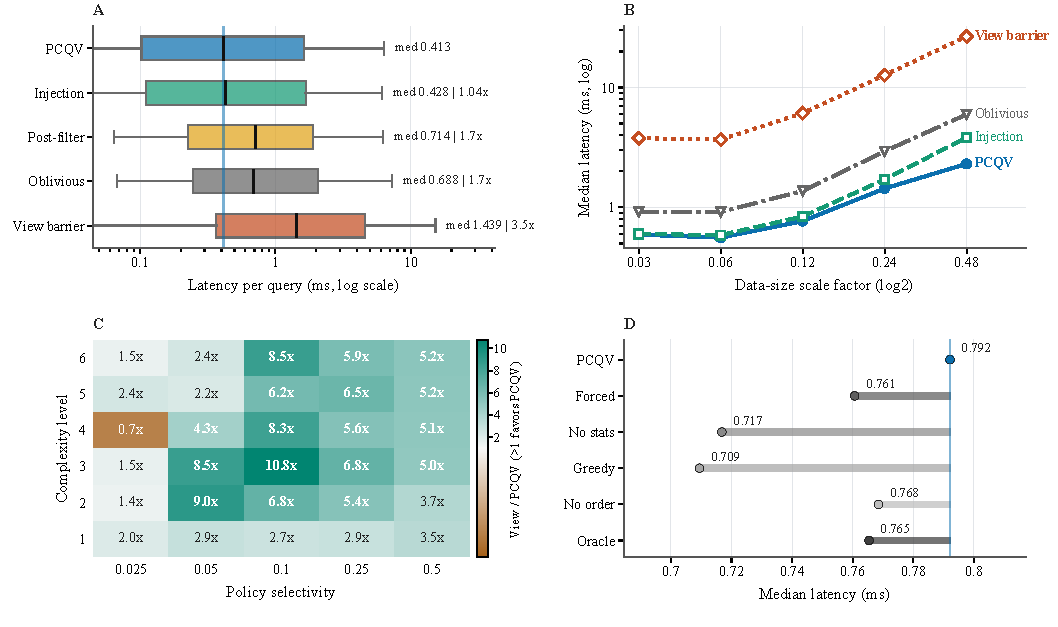
\includegraphics[width=\textwidth]{figures/fig_performance_suite.pdf}
\caption{Empirical summary generated directly from experiment outputs. (A) Safe-method latency distribution on a log scale; boxes show medians and interquartile ranges, whiskers show the 5th--95th percentiles, and fliers are hidden for print readability. (B) Five-size scale sweep on log-log axes. (C) View-barrier/\pcqv{} ratio over policy selectivity and complexity, with higher levels at top; values above 1 favor \pcqv{}. (D) Planner variants that separate protected-cardinality costing, greedy search, forced order, and oracle diagnostics.}
\label{fig:performance-suite}
\end{figure*}

\begin{table}[t]
\centering
\caption{Performance summary from 4,320 measurements. Diagnostics such as no-stats, forced order, and oracle order are reported in the ablation study.}
\label{tab:perf}
\begin{tabular}{lrr}
\toprule
Method & Median ms & P95 ms \\
\midrule
\pcqv{} & 0.413 & 6.369 \\
Injection & 0.428 & 6.152 \\
Oblivious & 0.688 & 7.285 \\
Post-filter & 0.714 & 6.268 \\
View barrier & 1.439 & 15.234 \\
No policy (diag.) & 3.558 & 21.569 \\
\bottomrule
\end{tabular}
\end{table}



The no-policy reference can be slower because policies filter data early; the fair comparison fixes protected semantics and compares only safe execution strategies.

Table~\ref{tab:byquery} reports representative query families chosen to cover both favorable and unfavorable cases. Q12 and Q16 are the new four-way stress cases; Q10 isolates ACL and masking without joins; Q11 adds an order-ticket bridge; Q5 remains a negative case where a safe view barrier can be competitive. These rows show that the contribution is not a single speedup number: the optimizer contract must explain when injection is enough, when barriers are too opaque, and when protected cardinality changes the best safe encoding.

\begin{table}[t]
\centering
\caption{Representative median latency by query template (ms).}
\label{tab:byquery}
\begin{tabular}{lrrrr}
\toprule
Query & \pcqv{} & Inject & Obliv. & View \\
\midrule
Q1 & 0.426 & 0.290 & 0.941 & 2.554 \\
Q5 & 1.668 & 2.030 & 1.988 & 0.502 \\
Q6 & 0.622 & 0.707 & 2.084 & 3.696 \\
Q10 & 0.124 & 0.193 & 0.158 & 0.254 \\
Q11 & 0.472 & 0.434 & 0.493 & 0.775 \\
Q12 & 0.496 & 0.652 & 0.755 & 3.324 \\
Q13 & 1.116 & 0.891 & 0.929 & 2.572 \\
Q14 & 0.217 & 0.246 & 0.290 & 0.441 \\
Q15 & 0.411 & 0.322 & 0.339 & 2.364 \\
Q16 & 0.994 & 0.742 & 0.824 & 3.451 \\
\bottomrule
\end{tabular}
\end{table}

\subsection{RQ3: Efficiency and Scalability Under Selectivity, Complexity, and Scale}
Fig.~\ref{fig:performance-suite}(C) and Table~\ref{tab:selectivitytable} show selectivity sensitivity. At very low selectivity, native predicate injection often has the lowest median latency because indexes prune the tenant slice. As selectivity grows, barriers and policy-oblivious forced order amplify intermediate tuples. \pcqv{} follows injection at low selectivity and the forced policy-aware order at wider slices.


\begin{table}[t]
\centering
\caption{Median latency by policy selectivity (ms).}
\label{tab:selectivitytable}
\begin{tabular}{lrrrr}
\toprule
Sel. & \pcqv{} & Inject & Obliv. & View \\
\midrule
0.025 & 0.055 & 0.053 & 0.178 & 0.062 \\
0.050 & 0.115 & 0.118 & 0.289 & 0.674 \\
0.100 & 0.384 & 0.374 & 0.498 & 2.272 \\
0.250 & 1.102 & 1.195 & 1.751 & 6.024 \\
0.500 & 2.556 & 2.589 & 3.472 & 11.901 \\
\bottomrule
\end{tabular}
\end{table}

Fig.~\ref{fig:performance-suite}(C) and Table~\ref{tab:complexitytable} show policy-complexity sensitivity. Tenant isolation is indexable, but purpose, clearance, cross-table guards, ACL disjunctions, and group thresholds shift protected cardinalities. Fig.~\ref{fig:performance-suite}(B) makes scalability explicit: the five-size CPU-safe scale sweep records \ScaleSweepRows{} measurements. At the largest sweep point, \pcqv{} median latency is \ScaleLargestPcqvMs{} ms, compared with \ScaleLargestInjectionMs{} ms for injection, \ScaleLargestObliviousMs{} ms for policy-oblivious forced order, and \ScaleLargestViewMs{} ms for view barriers; the view-barrier/\pcqv{} ratio is \ScaleLargestViewSpeedup{}$\times$.


\begin{table}[t]
\centering
\caption{Median latency by policy complexity (ms).}
\label{tab:complexitytable}
\begin{tabular}{lrrrr}
\toprule
Level & \pcqv{} & Inject & Obliv. & View \\
\midrule
1 & 1.024 & 0.942 & 1.254 & 2.377 \\
2 & 0.473 & 0.450 & 0.878 & 1.852 \\
3 & 0.223 & 0.291 & 0.483 & 1.062 \\
4 & 0.261 & 0.229 & 0.604 & 1.473 \\
5 & 0.326 & 0.320 & 0.602 & 1.255 \\
6 & 0.329 & 0.384 & 0.617 & 1.280 \\
\bottomrule
\end{tabular}
\end{table}


\begin{table}[t]
\centering
\caption{Policy-aware explanation for Q6 at selectivity 0.025 and level 1.}
\label{tab:planexample}
\begin{tabular}{lrr}
\toprule
Alias & Table rows & Protected estimate \\
\midrule
c: customers & 1,200 & 30.000 \\
o: orders & 5,000 & 125.000 \\
l: lineitem & 12,000 & 240.000 \\
p: products & 300 & 6.675 \\
\bottomrule
\end{tabular}
\end{table}

\subsection{RQ4: Planning Overhead, Cardinality, and Ablations}
Planning overhead is small relative to execution in this prototype, although not zero. Median compile/planning time is 0.157 ms for \pcqv{}, 0.060 ms for the forced policy-aware enumerator, and 0.015 ms for predicate injection over 1,536 planning measurements. The diagnostic oracle order costs 2.291 ms median because it issues actual-cardinality probes and is not used by the deployed method. The cardinality study reports median policy-aware Q-error 1.139 and P95 3.500 over 1,230 base-cardinality checks. A separate optimizer-search audit creates \OptimizerSearchCases{} visibility-capsule states with four to \OptimizerSearchMaxAliases{} aliases and exact left-deep search over as many as \OptimizerSearchMaxOrders{} alias orders. Greedy policy-aware search is suboptimal in \OptimizerSearchSuboptimal{}/\OptimizerSearchCases{} cases, with \OptimizerSearchMaxRegret{}$\times$ maximum regret, which supports the dynamic-programming candidate planner rather than a one-step heuristic whenever the protected search space is still tractable.

\begin{table}[t]
\centering
\caption{SQL compile/planning overhead.}
\label{tab:planning}
\begin{tabular}{lrr}
\toprule
Method & Median ms & P95 ms \\
\midrule
Injection & 0.015 & 0.031 \\
View barrier & 0.019 & 0.035 \\
\pcqv{} no stats & 0.036 & 0.210 \\
\pcqv{} forced & 0.060 & 0.692 \\
\pcqv{} & 0.157 & 1.274 \\
Post-filter & 0.050 & 0.085 \\
\bottomrule
\end{tabular}
\end{table}

Fig.~\ref{fig:performance-suite}(D) shows ablations over the \pcqv{} planner family. The no-stats and oracle variants are intentionally not presented as deployed methods: the former removes a visibility component and can win on short SQLite cells by avoiding planning work, while the latter uses measured protected cardinalities unavailable to an optimizer. Greedy search is fast but measurably suboptimal on the optimizer-search audit, which justifies exact DP for the tractable alias counts studied here. Predicate injection remains the main non-\pcqv{} competitor in Table~\ref{tab:perf}; the ablation's role is to separate safe candidate generation, cost visibility, search, diagnostics, and equivalence testing rather than to claim that one selectivity formula dominates every SQLite cell.


\subsection{RQ5: Failure Cases and Diagnostics}
Two diagnostic findings shape the paper. First, simple predicate injection is often strong on SQLite, so the evaluation treats it as a first-class competitor rather than a strawman. \pcqv{} instead treats injection as a safe candidate and reports where it is sufficient. Second, unsafe late aggregation can appear performant but is semantically wrong. It leaks or suppresses aggregate groups because rows that should be excluded by tenant, purpose, clearance, or cross-table guards have already contributed to group state. The mutation suite in Table~\ref{tab:failures} adds eight smaller faults to avoid a vacuous checker: dropping masks, tenant guards, purpose/owner guards, clearance/risk guards, region guards, cross-table guards, ACL exceptions, and group guards. The suite records both symmetric differences and violating candidate rows, so a reviewer can inspect whether a fault is undetected because it is semantically irrelevant for that generated case or because the checker missed a real discrepancy. The region mutation is a useful negative result: in this workload it is often subsumed by the ACL-or-region level, so the checker reports zero difference rather than inventing a violation.

\begin{table}[t]
\centering
\caption{Negative controls surfaced by the checker. Diff. counts symmetric output differences; viol. counts candidate rows absent from the reference.}
\label{tab:failures}
\begin{tabular}{lrrrr}
\toprule
Fault & Tests & Equiv. & Diff. & Viol. \\
\midrule
Late agg & 128 & 40 & 4,657 & 3,816 \\
No tenant & 42 & 4 & 2,928 & 2,539 \\
No purpose & 42 & 19 & 1,717 & 1,256 \\
No mask & 42 & 30 & 2,620 & 1,310 \\
No ACL & 42 & 30 & 464 & 464 \\
No clear & 42 & 16 & 325 & 202 \\
No cross & 42 & 32 & 18 & 14 \\
No region & 42 & 42 & 0 & 0 \\
No group & 42 & 36 & 134 & 134 \\
\bottomrule
\end{tabular}
\end{table}

Beyond speedups, the evaluation explains degradation: barriers hide interleaving opportunities, post-filtering carries raw attributes and delays guards, policy-oblivious orders ignore protected cardinality, and injection is fast when the engine exploits predicates but does not independently certify masks or aggregate guards.

\subsection{Lessons for Optimizer Design}
The evaluation suggests three lessons. First, policy transparency is more important than policy placement alone: a policy-aware optimizer should represent policies once and print several safe SQL encodings, while certificates expose enough information to reject a misplaced guard, mask, or release boundary. Second, policy-aware costing is a certified optimizer signal; protected cardinalities explain when barriers and policy-oblivious starts are fragile. Third, rewrite verification should be part of the optimizer workflow, because unsafe early aggregation is a familiar performance transformation applied at the wrong semantic boundary.

\subsection{Robustness, Scalability, and Transfer}
\label{sec:robustness}
The evaluation turns policy-aware optimization claims into executable obligations. Fixed workloads check plan behavior; TPC-H/SSB-style and JOB/IMDb-style schemas stress recognizable analytics; finite-model, SQL-feature, randomized-fuzzing, certificate, field-necessity, and bootstrap audits check semantics beyond one SQLite run. The contract is a portable efficiency/scalability interface: a DBMS, middleware optimizer, or governance-layer query generator would need to expose the same capsule fields and require each new operator to provide a protected denotation, rewrite preconditions, cost-visible state, and counterexample family.

\textbf{Data-engineering impact.} A platform team can audit this optimizer interface independently of a particular policy language. A governance layer compiles guards, masks, release checks, and protected selectivity once, exposes them as memo properties, and lets a cost-based optimizer choose among barrier, injection, post-filter, and forced-order encodings. The scale sweep shows the execution effect; the memo-property audit shows that the same visibility can be consumed by optimizer machinery rather than remaining a paper-only abstraction.

\textbf{Transfer path.} A DBMS or governance-layer optimizer can store capsule fields as memo properties or rule preconditions, feed protected selectivity into costing, and keep the protected-view oracle as a regression harness; the memo-property bridge audit turns this path into \MemoCandidateRecords{} executable records. New SQL features can follow the same discipline: specify the protected denotation, state admissible rewrites, identify cost-visible state, and add witness families before enabling the rule.


\section{Related Work}
\label{sec:related}
\pcqv{} builds on the ordinary optimizer substrate. Relational semantics, dynamic-programming optimization, Volcano/Cascades enumeration, and join-order search define the base machinery\cite{codd1970relational,abiteboul1995foundations,selinger1979access,graefe1993volcano,graefe1995cascades,chaudhuri1998overview,graefe1993query,ioannidis1990randomized,swami1988largejoins,steinbrunn1997heuristic}. Adaptive optimization, cardinality estimation, multiobjective planning, physical design, and access paths refine that machinery\cite{kabra1998midquery,babcock2005robust,leis2015job,leis2017lookingglass,kipf2019learnedcards,hilprecht2020deepdb,dutt2019selectivity,trummer2016multiobjective,chaudhuri1997autoadmin,bruno2005autoadmin,bayer1972btree,comer1979btree}. \pcqv{} asks what additional policy-visible state this substrate needs before a rewrite is admissible.

Predicate movement, user-defined-function rewrites, view-based answering, and unnesting provide the closest rewrite machinery\cite{hellerstein1993predicate,chaudhuri1996udf,levy1994predicate,chaudhuri1995views,goldstein2001views,halevy2001views,pottinger2001minicon,larson1985derived,ganski1987nested,neumann2015unnesting}. SQL-equivalence and learned-rewrite tools add validation and search for ordinary SQL denotations\cite{chu2017cosette,chu2017hottsql,zhou2019symbolic,wang2022wetune,zhou2023learnedrewrite,ding2024lia,wang2024qed}. \pcqv{} differs by making guards, masks, release boundaries, and protected selectivity explicit optimizer obligations rather than treating protected views as ordinary subqueries.

Database authorization, fine-grained access control, predicated grants, Hippocratic databases, row-level security, and purpose/consent policies define the enforcement setting\cite{stonebraker1974access,griffiths1976authorization,sandhu1996rbac,bertino2005database,rizvi2004fgac,kabra2006redundancy,lefevre2004disclosure,agrawal2002hippocratic,agrawal2003privacy,agrawal2005privacy,chaudhuri2007predicated,byun2008purpose,konstantinidis2022consent,dar2023rls,paduroiu2024membrane,xue2020guardspark,xue2023sparkac}. Privacy definitions and provenance explain adjacent semantics for disclosure and data dependence\cite{sweeney2002kanonymity,machanavajjhala2007ldiversity,li2007tcloseness,dwork2006calibrating,buneman2001provenance,cui2000lineage,green2007provenance}. \pcqv{} is not a new access-control model or policy language; it assumes such policies have been chosen and exposes the optimizer contract needed to preserve their protected denotation.

Generated-query testing and benchmark practice shape the evaluation methodology\cite{rigger2020pqs,rigger2020norec,rigger2020tlp,ba2023qpg,ba2024dqp,tpch,tpcds,oneil2009ssb,nambiar2006tpcds,pavlo2009benchmark,olston2008pig,armbrust2015sparksql,boncz2005x100,neumann2011compiling}. Relative to these lines, \pcqv{} is not a standalone equivalence prover or benchmark suite; it is the optimizer interface after a policy has been chosen: capsule fields become rewrite preconditions, protected selectivity becomes cost state, and negative controls make unsafe rules falsifiable.

\section{Conclusion}
\pcqv{} makes policy semantics part of query optimization rather than a hidden enforcement side effect. Visibility capsules record guards, dependencies, masks, release conditions, deterministic prefixes, and protected selectivities; certificates explain why a rewrite is legal; the planner uses the same state to choose among safe encodings. Across the reported workloads, this turns policy-constrained query processing into a checkable optimization problem: the system exposes why a plan is safe, why it is expected to be cheaper, and which artifact reproduces the claim. The practical consequence is a cleaner division of responsibility: a policy compiler owns protected denotation and mask obligations, an optimizer owns enumeration and costing, and a regression harness owns falsification. That separation also keeps the evidence reviewable: each reported speedup has a safe reference result, each unsafe shortcut has a negative control, and each admitted rewrite names the capsule fields it consumes. The claim remains bounded: \pcqv{} is the optimizer-facing layer for the studied settings, not a replacement for row-level security, consent systems, or equivalence provers. Future integrations should expose the capsule fields, define each new protected denotation, and keep the witness suite as a regression gate before enabling rules. A port therefore needs a protected-denotation contract and witnesses, not only an optimized SQL string. Because the contract is field-level, failures are local: a rejected plan points to a missing guard, mask position, release boundary, deterministic prefix, or stale protected-cardinality estimate, and the corresponding witness can be rerun without reinterpreting the policy stack. That endpoint keeps the central contract intact: cost-based choices are made only after protected semantics is explicit and each added rule remains witness-backed.

\clearpage

\section*{Guidelines for Artificial Intelligence (AI)-Generated Content}
AI was used only for language and grammar polishing.

\bibliographystyle{IEEEtran}
\bibliography{references}

\end{document}
